\documentclass[letterpaper,12pt]{article}
% define the title
\usepackage{xcolor,graphicx,subfigure}

\usepackage{epigraph}

% \epigraphsize{\small}% Default
\setlength\epigraphwidth{16cm}
\setlength\epigraphrule{1pt}
\usepackage[margin=1.25in]{geometry}

\usepackage{etoolbox}

\makeatletter
\patchcmd{\epigraph}{\@epitext{#1}}{\itshape\@epitext{#1}}{}{}
\makeatother\usepackage{algorithm}
\usepackage{multirow}
\usepackage{algpseudocode}
\begin{document}
% generates the title
\begin{titlepage}
\begin{center}

% Upper part of the page. The '~' is needed because \\
% only works if a paragraph has started.

\textsc{\huge Bad Commit Smells}\\[0.5cm]
\textsc{ Those Who Do Not Learn From Their Commit History Will be Doomed to Revert it}\\[1.0cm]


% Author and supervisor
\begin{minipage}{0.4\textwidth}
\begin{flushleft} \large
Steven \textsc{Johnson}
\end{flushleft}
\end{minipage}
\begin{minipage}{0.4\textwidth}
\begin{flushright} \large
Zach \textsc{Welch}
\end{flushright}
\end{minipage}\\[1.5cm]

\large University of Wisconsin \textsc{Madison}\\[1.5cm]

\begin{abstract}
On a given day, a large open-source Git Repository likely receives many pull requests, plenty of which are submitted by �untrusted� public members who have yet to contribute to the repository. With so much information to look up and code to test for managers of the repository, we have developed a method to extract metadata about commits and their messages, analyze this data using machine learning techniques, and determine which commits are suspect for introducing new bug(s). The accuracy of our classification method is verified using a number of open-source git repositories, including jedit, jquery, scala, and git itself. Our ensemble classifier correctly predicts bugginess of commits between 70 and 90\% of the time, outperforming the baseline of random weighted guessing by roughly 15 to 25\%. This tool furthers the goal of better directing the testing efforts of repository owners by providing recommendations about suspect commits and also seeks to inform contributors in ways to improve their commit structure to make their commits less suspect.
\end{abstract}


\vfill

% Bottom of the page
{\large \today}

\end{center}
\end{titlepage}

% insert the table of contents
\tableofcontents
\listoffigures
\listoftables
\epigraph{Yeah Science!!}{ \textup{Jesse Pinkman}}

\section{Introduction}
 
\section{Related Work}
Using version control system history to aid the development process is not a new idea;  the wealth of data that repositories store makes them very attractive artifacts to researchers who want to understand and improve the ways in which code is written.  In the last ten years a good deal of work has gone into trying to use repository data to make various aspects of the development process easier [3]. In the early 2000s Zimmerman et al [1] and Ying [2] developed systems to mine version history to make suggestions on potential locations to make changes based on recent alterations to versioned files. Their results were very interesting,  reliably finding associations between sections of code and between code and documentation. 

  A common goal in many projects involving software repositories is attempting to predict the bugginess of future code using some set of metrics. A wide variety of metrics have been researched, including code churn [6], association of changed files, distance between team members [7], and commit size[8]. Recent research has also been done to analyze the accuracy of predicting one repository�s future defects using a different repository�s past history [12].   Work has also been done on analyzing characteristics of bugs and bug fixes[9] [10]
  
There has also been some work in attempting to automatically infer which past commit introduced a bug.  Originally described in [CITE], the SZZ algorithm uses keywords to find bug fixes, and then uses the version system�s blame feature to find which commits last touched the code this bug fix attempted to fix.  Future improvements were also made by [CITE], which we discuss in detail later.

Some work has also been done by this group at attempting to use machine learning techniques to predict the bugginess of future commits.  Our work differs from theirs in several ways, namely that their work focuses much more heavily on analysis of committed code, which we generally ignore in favor of the attributes and message of a commit.    
\section{Approach}
\subsection{Mining Git Repositories}
We mined eight open-source repositories hosted on Github.com for features to serve as our testing data sets (Figure 1). The repositories are quite varied; they range in size from around 2000-30000 commits and in age from roughly 3-13 years. We extracted two sets of features about commits from each repository: commit attributes and message attributes. Commit attributes are information about a commit excluding actual analysis of the code or the commit message. Examples of commit attributes we extracted are the number of lines added, the number of lines removed, the contributor, the length of the comment, the day of the week of the commit, and the number of files altered. The commit message attributes we selected are the frequency of words, grammatical correctness, and readability and stylistic metrics of the message. We used the Kincaid metric for readability [CITE], diction, a unix command line tool, to quantify style (triteness, over-wordiness) [CITE], and Queequeg to test the degree of grammatical correctness [CITE] for each commit message. Our analysis of the commit messages assumes they are written in English.
\subsection{Automatically Classifying Past Commits}
To create a classification model from these features, we required a �ground truth� about whether or not each commit was bug inducing. We used a modified version of a heuristic from [CITE] to determine the set of commits for each repository that were bug inducing. This technique works by first identifying the set of commits in the repository which are bug fixes. Our modification of the heuristic accomplishes this with an analysis of the commit message looking for words such as �bug� or �fix�, or for strings of numbers and letters that appear to be bug-tracking numbers. After defining this set of bug fix commits, we process each commit individually, identifying hunks of source code that the commit altered. For each hunk, we then flag as bug-inducing the most-recent commit before our bug fix commit which altered that hunk of code. This analysis is conducted using a annotation ASDFASDFASF (graph/tree) search [CITE]. Obviously, this heuristic is imperfect�it depends on bug fix commits being atomic and on bugs being discovered and fixed immediately after their introduction. However, it works well in practice and serves as a good estimation for which commits are bug inducing, so we adopted it. (ASDFASDFSAF how do we know this????)

\subsection{Features}
With features extracted and a bugginess classification in hand for each commit for our selected repositories, we have the input prepared for constructing, training, and validating a machine-learning algorithm. The algorithm we selected to predict bugginess is an ensemble classifier, or in other words an aggregation of the outputs of several machine-learning algorithms (see Table 1). (ASDFASDFSDF list of our ml algs and perhaps their parameters??) The tuning of this method is an iterative process involving selecting the ideal set of features to train and test on, the sizes of both the training and testing datasets, and the machine-learning algorithms and their parameters to serve as initial classifiers. A list of features we examined, with those selected for the current version of our ensemble classifier highlighted, is found in Table 2.

\subsection{Machine Learning Algorithms}
\subsection{Pull Requests}
\section{Results}
\subsection{Data}
\subsection{Feature Analysis}
We went through several iterations of features to represent commits; we will briefly touch here on the features that did not work well before continuing to a more lengthy discussion of the features we actually used.  Our first attempt at classifying commits attempted to cast this prediction problem as equivalent to catching email spam.  A simple way to predict that an email is to train on the individual words in spam email.  The more a word is associated with being seen only in spam email, the more likely an email containing that word is spam.  We attempted to apply this to commits by training a Naive Bayes learner on the words of a commit messages. This turned out to be a not-very-good idea, with results about as good as randomly guessing clean or buggy.  Abandoning the buggy commit as email spam metaphor, we decided to look at attributes of the commit.   

   The features we chose to represent our commits are fairly simple ones; of the commit attribute data we use, only the day of the week required any computation.  Most of these attributes are presented to the user by git when they make a commit.  We did some initial testing with a decision tree learner, inspecting changes in results while testing differnt subsets of features.  We also manually kept track of which features were pruned from the tree, which indicates they are less informative.   We concluded Time and Date commit data is not very informative for the open source projects we chose to study.  Year and Month are too large to contain much signal, day of month and minute are too specific.  Because hour is not stored in local time and the generally distributed nature of these projects, we did not find Hour to be an informative feature.  It is possible that these features could be more valuable in a highly centralized development structure, where there is extra knowledge of development schedules and other information, but without any additional knowledge, we decided to ignore specific time-date data.  


\subsection{Testing Methodology}

To test the effectiveness of our feature selection, we mined features from eight open source repositories.  We attempted to choose projects with different life spans and applications to make our results more generalizable.  The list of projects mined, their number of commits, and the percentage of those commits we found to be buggy are in table {CITE}.

\begin{table}[h]
\begin{center}
    \begin{tabular}{ | c | c | c | c | c |}
    \hline
    Repository & Start Date & $\#$  Commits & $\#$ Buggy  Commits & \% Buggy \\ \hline
    one     & June 2008   &   8179 & 2744 & 33.6 \\ \hline
    cyclus & March 2010 &  2162 & 1071 & 49.5 \\ \hline
    git        & April 2005    &   28788 & 10682 & 37.1 \\ \hline
    jedit &Sept 1998 &  6890 & 3190 & 46.3 \\ \hline
    jquery     & March 2006   &   5608 & 3074 & 54.8 \\ \hline
    puppet & April 2005 &  12174 & 4812 & 39.5 \\ \hline
    scala     & Feb 2003   &   20398 & 9584 & 47.0 \\ \hline
    scipy & Feb 2001 &  10035 & 3252 & 32.4 \\ \hline        	
    \end{tabular}
\end{center}\caption{Mined Repositories}
\label{tab:repos}
\end{table}


  For each repository we mined, we took the year of 2013, regardless of its size, to be our test set.  The reasoning behind this is that in practice, users will want to classify new commits as they come in, and the most recent year of commits were the best fit of the data we had. Notice due to the way our heuristic works (start at a bug fix and work back) our test set is likely to contain more false negatives because the bug fixes have potentially not been written yet.  However, in practice this will also be the case so we feel this should not unreasonably skew our results.
 \begin{figure}[h]
\centering
	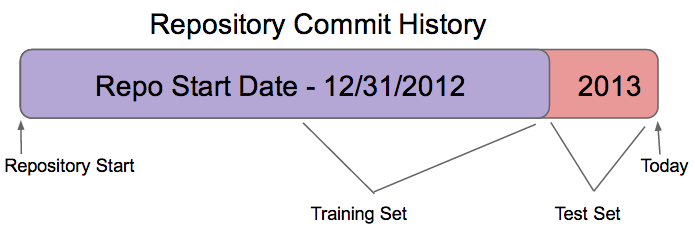
\includegraphics[width=0.75\textwidth]{images/history}
\caption{Testing and Training Sets}
\label{git_comp}

\end{figure}

 	For training data, we took commits from the final day of 2012 back six months, one year, two year, and to the start of the repository.  The goal here is to see how our results change with more data to train on (and potentially overfit to). 
	
	
	\begin{table}[h]
\begin{center}
    \begin{tabular}{ | c | c | c | c | c |c|}
    \hline
    
Repo & Test Set & 6Mo Train  & 1 Yr Train   & 2 Yr Train & All Train \\ \hline


one &  2304  &  1190 &  2423 & 4367  &  5874 \\ \hline
cyclus & 546  & 389  & 1231  & 1524  & 1616 \\ \hline
git & 2916  & 1369  & 2630  & 5129  & 25869 \\ \hline
jedit & 165  & 301  & 760  & 1401  & 6725 \\ \hline
jquery & 898  & 592  & 925  & 1934  & 4695 \\ \hline
puppet & 2195  & 980  & 2130  & 3854  & 9979 \\ \hline
scala & 1752  & 1347  & 2983  & 5080  & 18644 \\ \hline
scipy & 1873  & 546  & 1130  & 1786  & 8162 \\ \hline


 
\end{tabular}
\end{center}\caption{Size of Training and Test Sets}
\label{tab:size}
\end{table}

	\begin{table}[h]
\begin{center}
    \begin{tabular}{ | c | c | c | c | c |c|}
    \hline
    
Repo & Test Set & 6Mo Train  & 1 Yr Train   & 2 Yr Train & All Train \\ \hline


one  & 23.1 & 26.4 & 30.2 & 35.4 & 37.7 \\ \hline 
cyclus  & 30.6 & 44.4 & 50.6 & 54.9 & 55.9 \\ \hline 
git  & 13.9 & 22.1 & 22.5 & 23.4 & 39.7 \\ \hline
jedit  & 6.7 & 13.9 & 24.7 & 23.1 & 47.3 \\ \hline
jquery  & 35.7 & 43.2 & 46.6 & 53.9 & 58.6 \\ \hline 
puppet  & 18.7 & 20.0 & 26.1 & 29.1 & 44.1 \\ \hline 
scala  & 27.2 & 45.3 & 48.8 & 50.3 & 48.9 \\ \hline 
scipy  & 18.8 & 23.6 & 23.6 & 24.7 & 35.5 \\ \hline
\end{tabular}
\end{center}\caption{Bugginess of Training and Test Sets}
\label{tab:buggy}
\end{table}

\subsection{Learner Accuracy}

 \begin{figure}[h]
\centering
	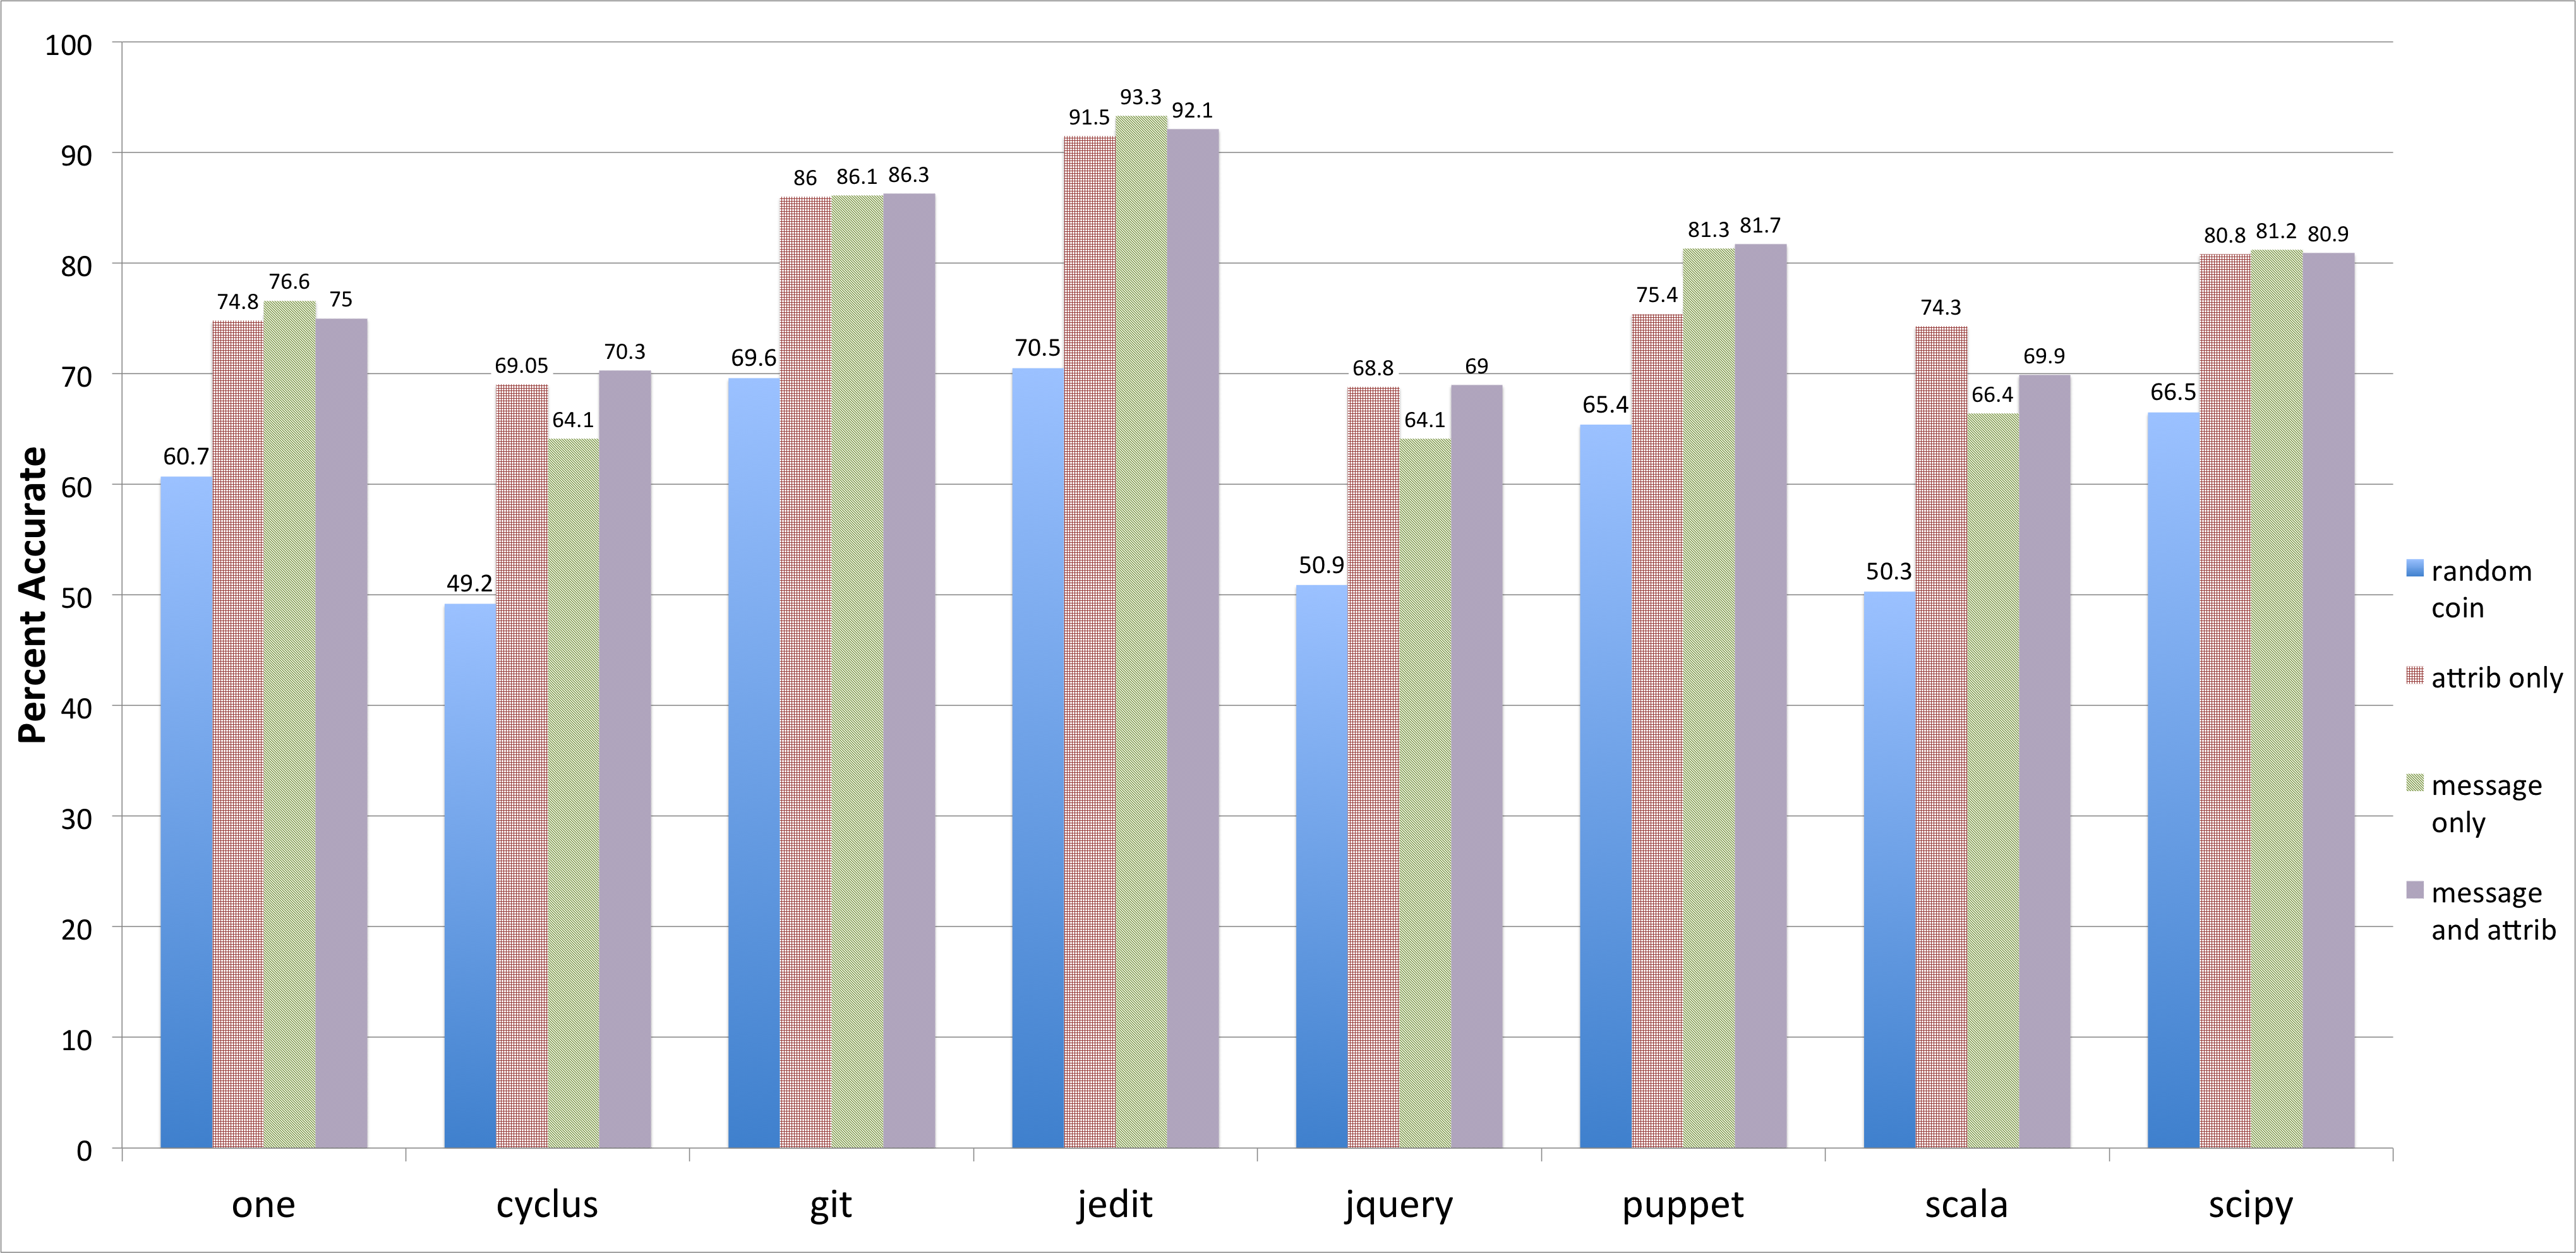
\includegraphics[width=0.75\textwidth]{images/learner_comp}
\caption{Comparison of Feature Results - 6 Months}
\label{git_comp}

\end{figure}

\subsection{Training Set Variation}

 \begin{figure}[h]
\centering
	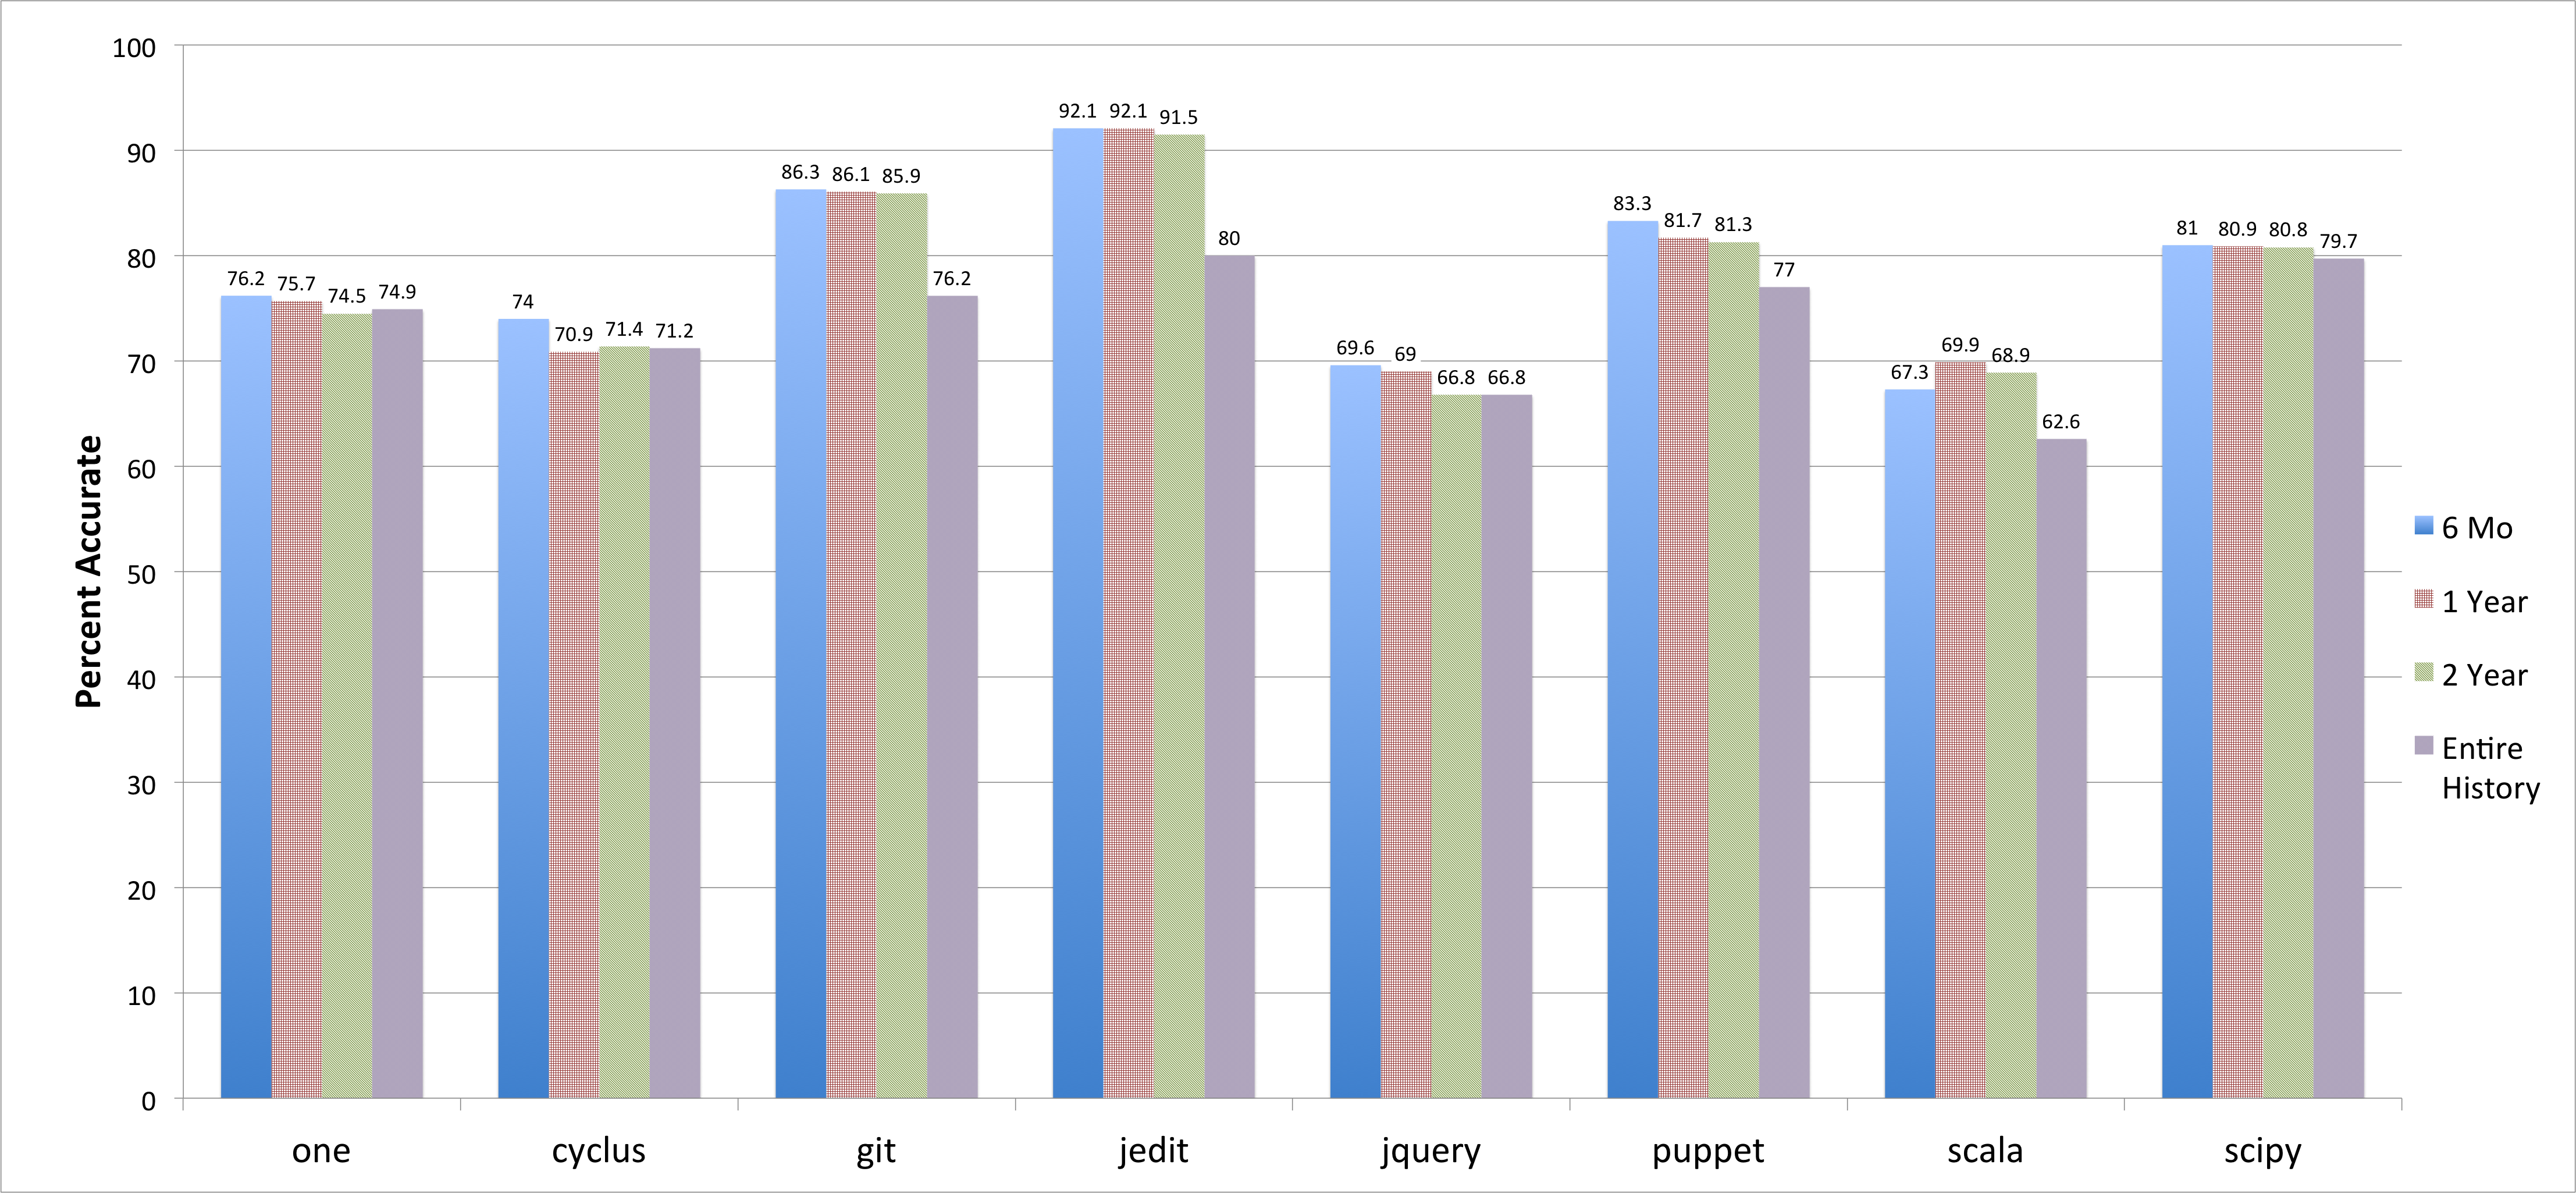
\includegraphics[width=0.75\textwidth]{images/time_comp}
\caption{Training Data Size - Message and Attributes}
\label{git_comp}

\end{figure}

\subsection{Cross Repository Training}

Six months to a year of repository data before being able to use a tool seems like a fairly high price of admission.  Being able to substitute another repository�s history for your own with little to no hit in accuracy seems like it would make our tool more applicable.  Furthermore, what does this say about commits if commits from two unrelated repositories are similar enough that one can be used to train the other?  To answer these questions, we decided to use git�s commit history to train our learner and test on the other seven repositories.  Git was chosen because it was the repository with the best nontrivial performance.  In order for training and testing data to be compatible, the user feature had to be removed from both data sets. 

 \begin{figure}[h]
\centering
	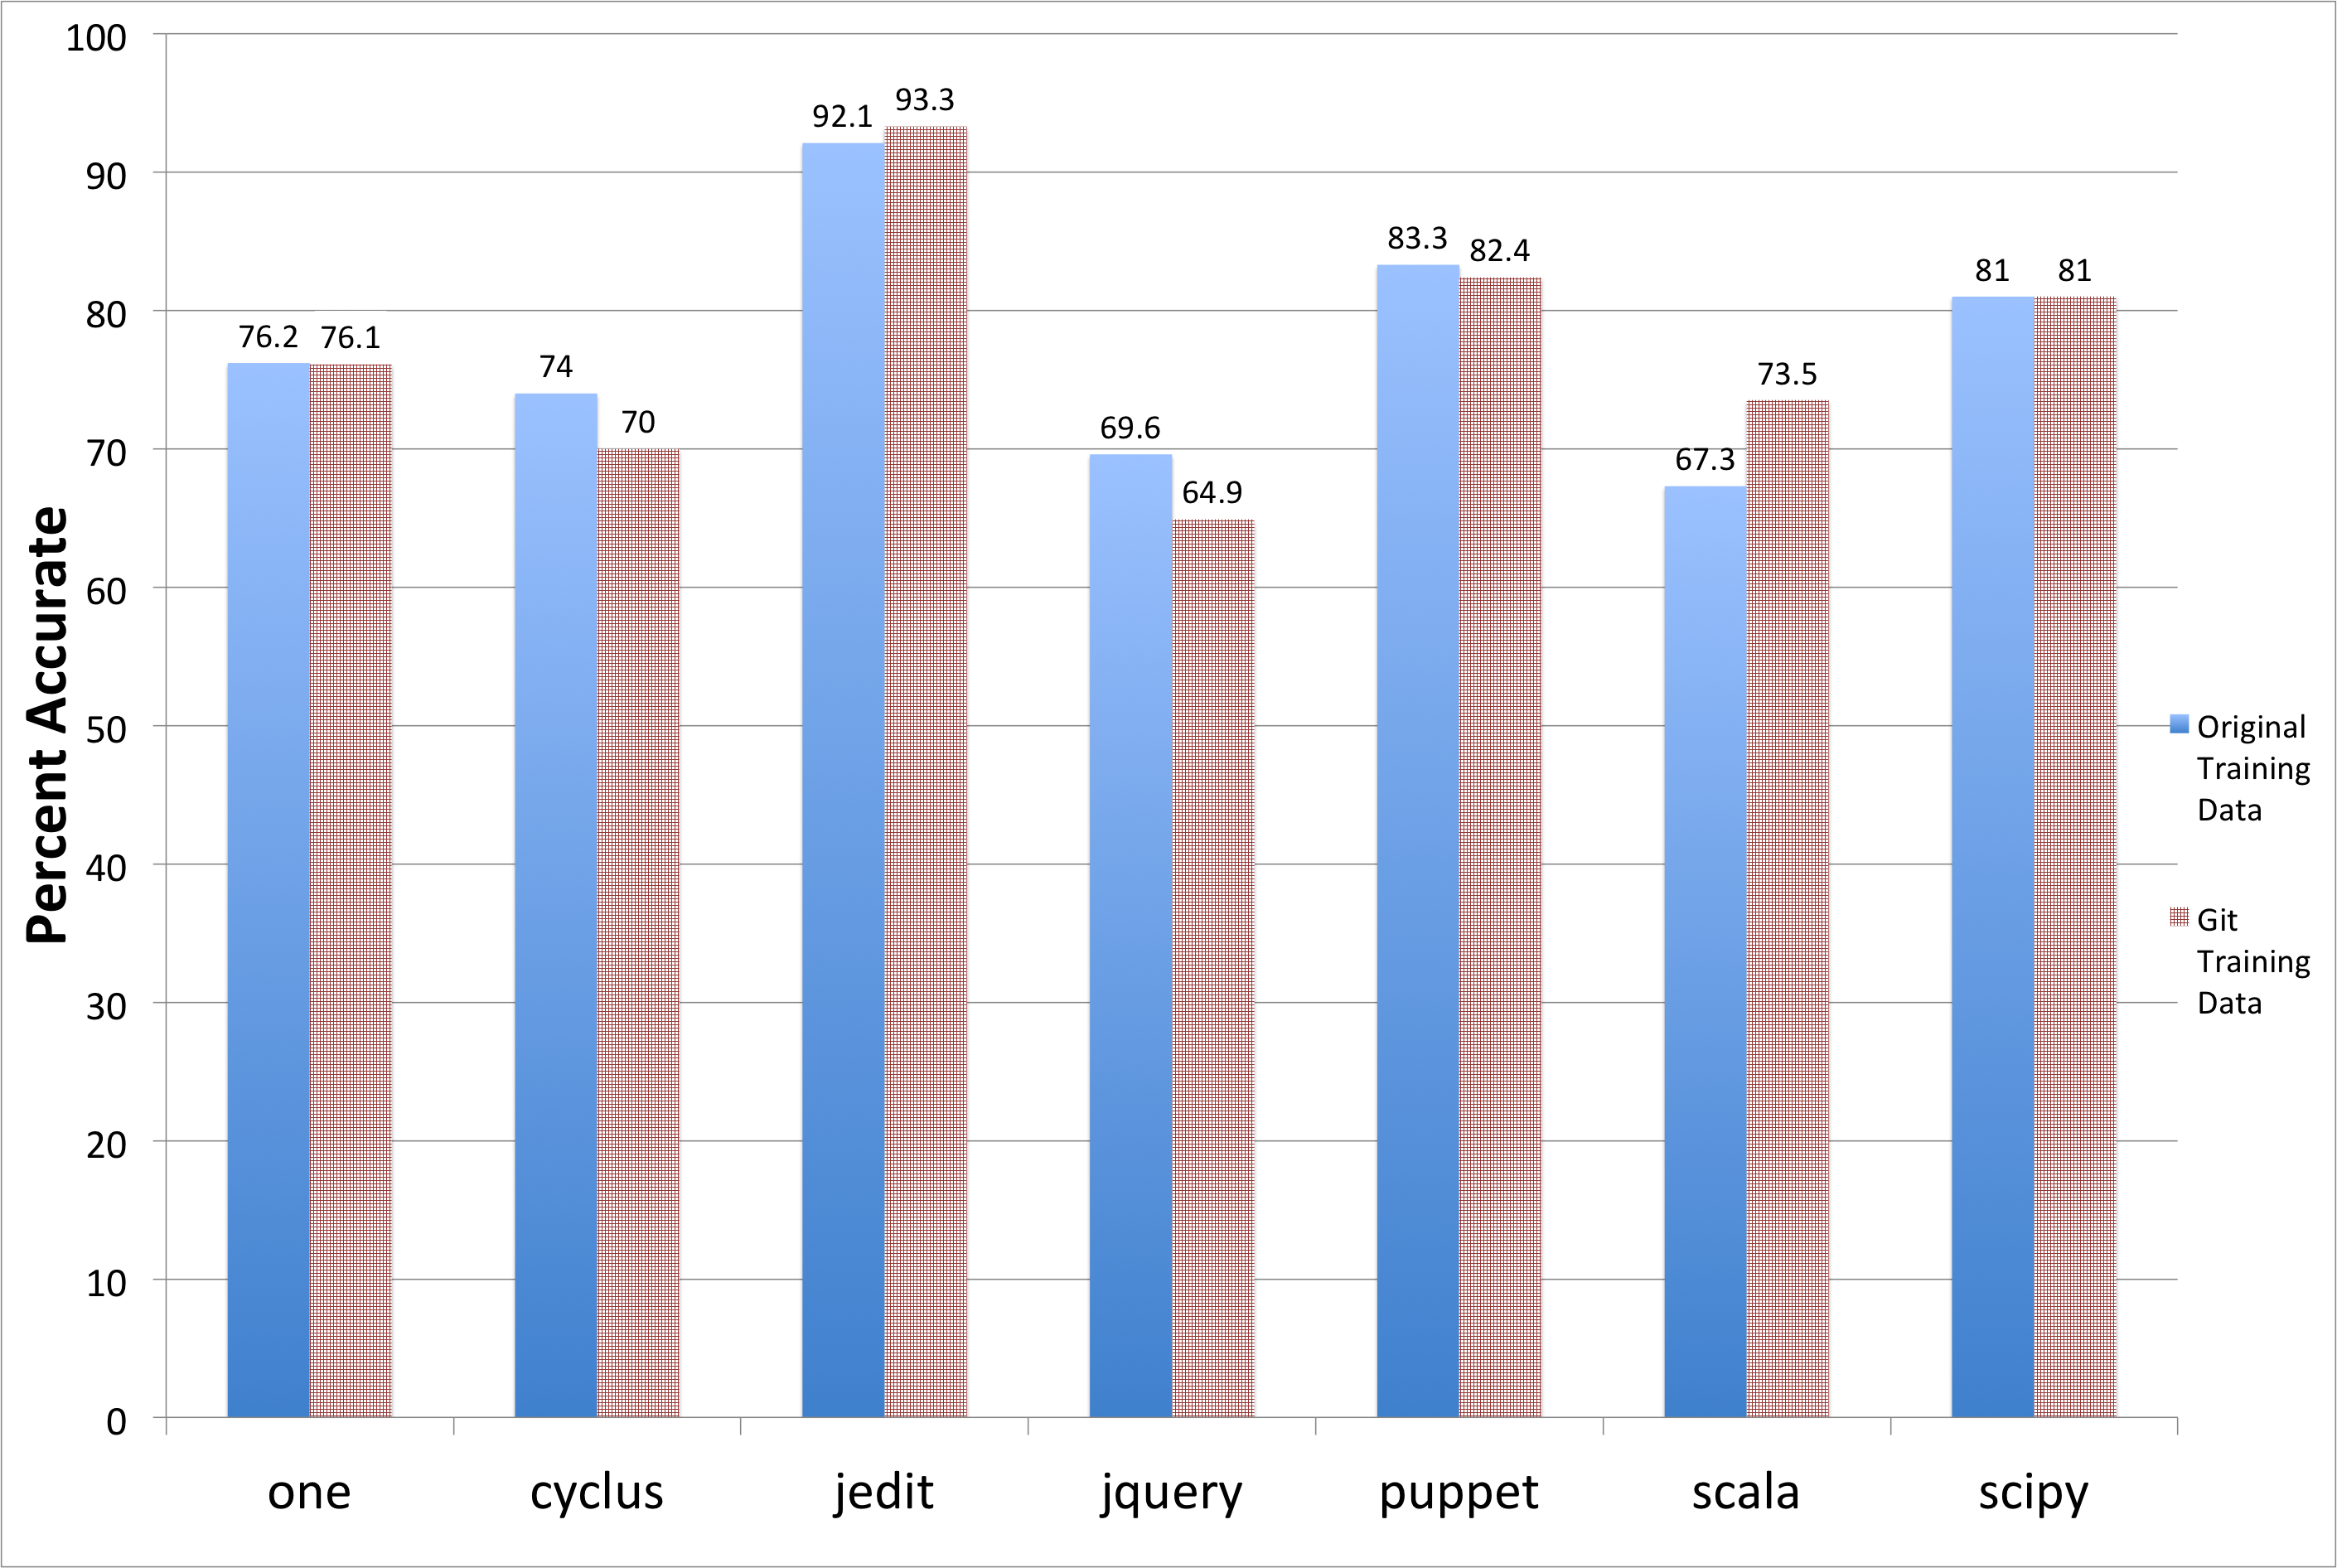
\includegraphics[width=0.6\textwidth]{images/git_comp}
\caption{Training With Git - 6 Months, Message and Attribute Data}
\label{git_comp}

\end{figure}

In general, results tended to be comparable to those using their respective data sets.  The git learner accuracies displayed the same trend of slow decrease as training data size increased, with a noticeable drop when all training data was used.  As Table [CITE] shows, cyclus and jquery see drop offs of about four percentage points, while scala performs six percentage points better.  The other four repositories stay essentially the same, with some minor variation.  Interestingly, the git trained learner is able to slightly improve on the always-guess-clean jedit learner even though the git training data is three times as buggy as the jedit test data.  

This comparable performance indicates to us that using a learner trained on another repository is a valid proxy for repositories that do not have their own history.  It also seems that the distribution of message and commit attribute features we use do not vary much across repositories.  More work would need to be done to give such a claim actual weight, but if our features have global, general boundaries, could we use this information in some kind of prescriptive fashion, a la �keep your commits to X lines added if possible�. Or would knowledge and enforcement of this information simply shift the boundary? 

\subsection{Threats to Validity}

There are several potential threats to the validity of our results.  The heuristic used in classifying past commits represents a multifaceted threat.  First, though [CITE] has presented some evidence that this method works well in practice, there is no evidence to support that these results generalize well.  As we mined neither of the two projects they studied, it is possible that our approximation of the true distribution of clean and buggy commits is flawed.  Even if we had mined those repositories, it is possible in the eight years between the writing of [CITE] and now that the heuristic does as well.  Another potential problem this heuristic introduces is that our ensemble learner is attempting to learn this approximation.  If the approximation does not closely match the actual distribution, then the results we present are in no way an indication of how our tool would perform against actual commits.

Another potential threat is the repositories we chose.  While we attempted to pick a representative sample of the open source projects in development, this excludes closed source projects. Also, we only mined english-speaking repositories, which is required by our heuristic classification and all of our message features.  We made no attempt to take into account differences and eccentricities of the individual repositories we did mine.  It is possible (even likely) that these eccentricities are to account for the variation between repositories.   

\section{Concluding Remarks}

% references section

\addcontentsline{toc}{section}{Bibliography}
\begin{thebibliography}{99}
\end{thebibliography}



% that`s all folks
\end{document}



